\section{Ein Überblick zu Recommerce und Preisstrategien}
Nicht erst seitdem es Online-Marktplätze gibt, ist die Festlegung von Preisen eine zentrale Herausforderung im Geschäftsbetrieb.
Durch Online-Marktplätze hat allerdings die Intensität des Wettbewerbs erheblich zugenommen, da Konkurrenzangebote leicht einsehbar sind und Preise in hochfrequentem Tempo gesetzt werden können.
Zudem müssen alle Produkte des meist sehr breiten Angebots in Abhängigkeit der Marktsituation dynamisch eingepreist werden.
Diese Gründe motivieren automatische Preisfindung, da menschliche Branchenexperten mit der Anpassung der Preise schlicht nicht mehr schritthalten können.

Eine weitere Schwierigkeit kommt im sogenannten Recommerce hinzu.
Recommerce beschreibt laut \cite{RecommerceDefinition} den Rückkauf, die Aufwertung und den Weitervertrieb von gebrauchten Produkten im Internet.
Gerade mit Blick auf die ressourcenintensive Modebranche verspricht Recommerce eine Steigerung der Nachhaltigkeit durch Einführung einer Kreislaufwirtschaft.
Wer einmal ein Produkt gekauft hat und als Eigentümer es irgendwann nicht weiter besitzen möchte, bekommt die Möglichkeit, durch Rückverkauf des Produktes etwas Geld einzunehmen.
Die gebrauchten und ggf. aufgewerteten Produkte werden dann zu niedrigeren Preisen weiterverkauft.
Zur Herausforderung, neue Produkte einzupreisen, kommt also noch hinzu, Preise für gebrauchten Produkte und die Rückkaufpreise festzulegen.
Dabei müssen auch Nebenbedingungen wie Lagerkosten beachtet werden, wodurch sich ein kompliziertes Problem ergibt.
\mbox{Abbildung \ref{graphic:MarketOverview}} zeigt eine grafische Visualisierung des in dieser Arbeit untersuchten Duopolszenarios.

\begin{figure}[htb]
	\centering
	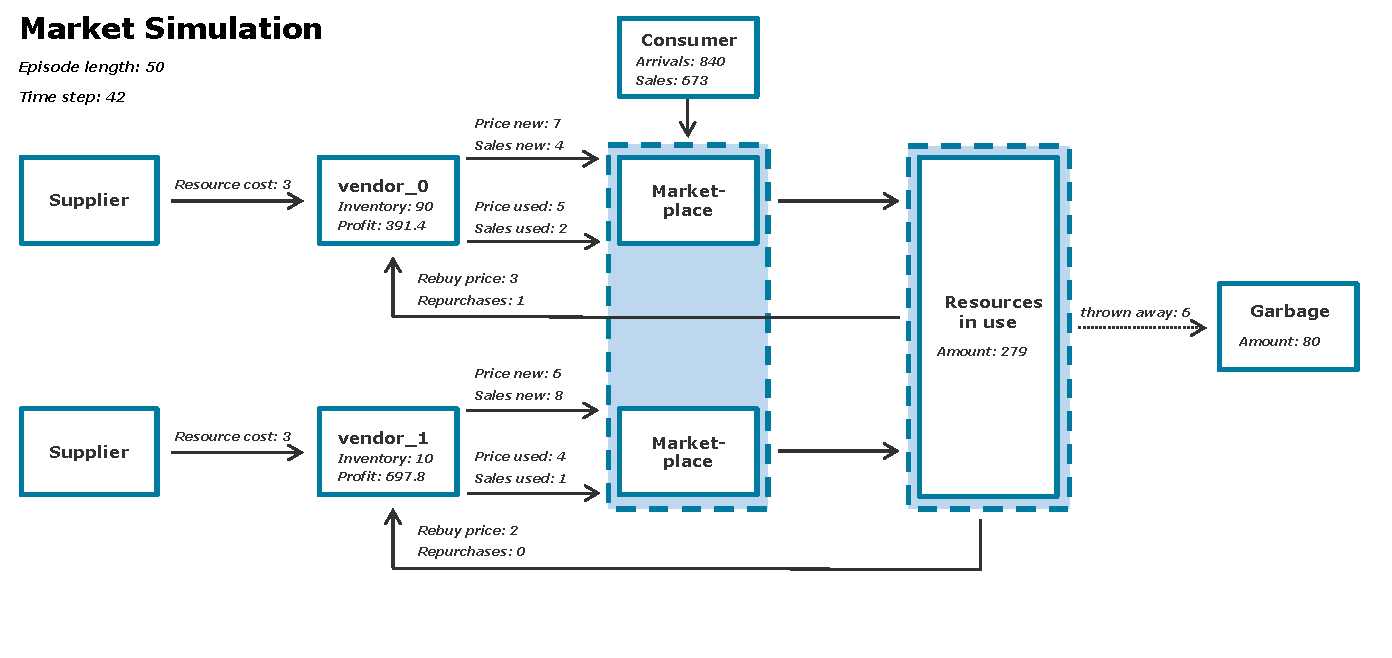
\includegraphics[width=\textwidth]{introduction/MarketOverview_042.pdf}
	\caption{
		Zwei Konkurrenten (vendor\_0 und vendor\_1) bieten die gleiche Produktlinie an.
		Beide legen Preise für ihre neuen und gebrauchten Produkte fest.
        Die Kunden (Consumer) entscheiden dann, ob und bei wem sie kaufen.
        Neuprodukte werden zu einem festen Preis vom Zulieferer (Supplier) eingekauft.
		Die Eigentümer der im Gebrauch befindlicher Produkte (Resources in use) haben die Wahl, ob sie das Produkt an einen der Händler zurückverkaufen.
        Sie können ihr Produkt auch trotz der Rückkaufangebote wegwerfen, sobald sie es nicht länger besitzen wollen.
	}
	\label{graphic:MarketOverview}
\end{figure}

Die Herangehensweisen für das Dynamic Pricing, die heute in der Geschäftswelt genutzt werden, basieren vor allem auf regelbasierten Strategien.
Dafür erstellen Marktexperten Heuristiken, die auf Erfahrungen und angestellten Überlegungen basieren.
Auf diese Art können durchaus gute Preisstrategien erstellt werden.
Allerdings werden dafür einerseits qualifizierte Marktkenner benötigt, und andererseits sind die Lösungen sehr speziell auf ein Marktszenario zugeschnitten.
Verändern sich die Umstände oder soll die Lösung für einen neuen Markt aufgesetzt werden, so muss der gesamte manuelle Prozess erneut durchlaufen werden.

Reinforcement Learning (RL) ermöglicht, nur auf Grundlage eines Marktes durch Ausprobieren und Sammeln von Erfahrung eine Preisstrategie zu optimieren.
Das Training geschieht dabei üblicherweise in einer Simulation, da auf echten Märkten durch das notwendige Ausprobieren ein erheblicher finanzieller Schaden entstünde.

Weil es sehr viele unterschiedliche RL-Algorithmen gibt, ist es eine interessante Frage, welche Vor- und Nachteile die einzelnen Algorithmen auf einem Recommerce-Markt haben.
Einen solchen Vergleich herzustellen, ist Ziel dieser Arbeit.
Zunächst wird das zu untersuchende Marktszenario in Abschnitt \ref{section:markov} als Markov-Entscheidungsprozess formalisiert und in Abschnitt \ref{section:rulebased} eine regelbasierte Strategie eingeführt.

\section{Der Markt als Markov-Entscheidungsprozess}
\label{section:markov}
Der Recommerce-Markt wird hier als Markov-Entscheidungsprozess modelliert.
Es wird zunächst das Duopolszenario eingeführt.
Dazu wird die Zeit in gleich lange Abschnitte diskretisiert.
Vor jedem Schritt wird dem Agenten der Zustand des Marktes präsentiert.
Daraufhin setzt der Agent seine Preise, die für den Rest des Schrittes gelten.
In der Übertragung eines echten Marktes könnte ein Schritt zum Beispiel einer Stunde oder einer Minute entsprechen.
Eigentlich soll die Optimierung für einen \textit{infinite horizon} stattfinden.
Das bedeutet, dass nicht auf einen festen Zeitraum hin optimiert wird.
Stattdessen wird auf ein langfristig profitables Equilibrium hingearbeitet.
Um allerdings das Problem für Training und Analyse handhabbar zu machen, werden Episoden betrachtet, die aus $n_{ep} \in \mathbb{N}$ Schritten bestehen.
Dieses $n_{ep}$ wurde in der Standardkonfiguration mit 500 so groß gewählt, dass der praktische Unterschied zu einer infinite-horizon-Betrachtung nur gering ist.

Das hier eingeführte Modell simuliert einen Recommerce-Markt mit zwei konkurrierenden Anbietern.
Der Markt soll fair und symmetrisch sein, was bedeutet, dass beide Anbieter die gleichen Produkte verkaufen, gleiche Beliebtheit haben, abwechselnd und für die gleiche Länge die Preise setzen und die gleichen Kosten haben.
Der erste Anbieter erneuert seine Preise stets zu Beginn jedes Schrittes, sein Wettbewerber nach der Hälfte des Schrittes.
In beiden dieser Phasen kommen gleich viele Kunden.
Damit können die Gewinne der beiden Anbieter direkt verglichen und auf die Güte der Preisstrategien geschlossen werden.
Zum Markov-Entscheidungsprozess wird der Markt, wenn er aus der Sicht eines der beiden Anbieter betrachtet wird, während der andere Anbieter ein Teil der Umgebung ist.
Das Verhalten des Konkurrenten kann deterministisch oder stochastisch sein.
Soll die Markov-Eigenschaft erfüllt werden, darf es sich aber während des Trainings und der Analyse nicht ändern.

Bei der folgenden Notation werden die Anbieter mit 1 und 2 indiziert.
Dabei ist 1 der Anbieter, aus dessen Sicht das Marktgeschehen abläuft.
Die in dieser Arbeit verwendeten Standardwerte für die Marktparameter sind im Anhang in der Tabelle \ref{tab:default_parameters} aufgeführt.

Für den Anbieter $i\in\{1, 2\}$ müssen in Abhängigkeit des Zustandes drei Preise gesetzt werden:
\begin{enumerate}
	\item für gebrauchte Produkte der Produktlinie ($p_{i, gebraucht}$),
	\item für diese Produkte in neu ($p_{i, neu}$) sowie
	\item den Rückkaufpreis ($p_{i, re}$), für den von einem Eigentümer gebrauchte Produkte zurückgekauft werden.
\end{enumerate}
Alle drei Preise bewegen sich zwischen 0 und dem maximal möglichen Preis $p_{max} \in \mathbb{N}$.
Damit ist der (stetige) Aktionsraum als $\mathcal{A}_\mathbb{R}=[0{,} p_{max}]^3$ definiert.
Alternativ lässt sich der Aktionsraum auch mit diskreten Preisstufen als $\mathcal{A}_\mathbb{N}=\{0{,} 1, \ldots, p_{max}\}^3$ definieren.
Die diskrete Formulierung schränkt deutlich stärker ein, ermöglicht aber (prinzipiell) exakte Lösungen, wie sie in Abschnitt \ref{section:dp} vorgestellt werden.
Zudem unterscheiden sich die Reinforcement-Learning-Verfahren für diskrete und stetige Aktionsräume.

In jedem Schritt besucht eine gerade natürliche Zahl $k$ an Kunden den Marktplatz.
Dabei treffen immer $k / 2$ Kunden auf den Marktzustand, in dem der erste Anbieter seine Preise aktualisiert hat und die alten Preise des zweiten Anbieters anliegen.
Die anderen $k / 2$ Kunden bekommen die unveränderten Preise des ersten Anbieters und die neuen Preise des zweiten Anbieters.
Die Kunden bewerten für sich die Angebote und treffen eine von fünf möglichen Entscheidungen.
Entweder kaufen sie kein Produkt, oder das gebrauchte oder neue bei einem der Anbieter.
Das Kaufverhalten ist aber keinesfalls homogen.
Es wird stark durch die Preise beeinflusst, aber unterschiedliche Kunden haben unterschiedliche Erwartungen, unterschiedliche Konsumgewohnheiten oder unterschiedliche Einstellungen zu Nachhaltigkeit.
Deshalb wird eine Wahrscheinlichkeitsverteilung des Kaufverhaltens für die fünf Optionen erstellt, aus der dann für einzelne Kunden gesampelt wird.
Das geschieht, indem für die einzelnen Optionen Präferenzen aufgestellt werden, aus denen dann per Softmax die Zähldichte der Wahrscheinlichkeitsverteilung berechnet wird.
Dabei wird die Präferenz für das Nichtkaufen auf 1 festgelegt.
Die Präferenz, das Neuprodukt bei Anbieter $i\in\{1, 2\}$ zu kaufen, lautet
\begin{equation}
	\sigma_{kunde, neu, i} = \frac{10}{p_{i, neu} + 1} - \exp{(p_{i, neu} + 1 - 0{,}8 p_{max})}.
\end{equation}
Das Kaufen eines Gebrauchtproduktes bei Anbieter $i\in\{1, 2\}$ wird auf
\begin{equation}
	\sigma_{kunde, gebraucht, i} = \frac{5{,}5}{p_{i, gebraucht} + 1} - \exp{(p_{i, gebraucht} + 1 - 0{,}5 p_{max})}
\end{equation}
festgelegt.
Die Addition der Preise mit eins verhindert Nulldivision.

Die Präferenz für eines der Angebote basiert also hauptsächlich auf dem Preis-Leistungs-Verhältnis.
Gebrauchten Produkten wird dabei 55\% der Wertschätzung im Vergleich zu Neuprodukten entgegengebracht.
Zusätzlich sinkt die Präferenz deutlich, wenn der Preis $0{,}5 p_{max}$ bei Gebraucht- und $0{,}8 p_{max}$ bei Neuware überschreitet.
Das modelliert die grundsätzlich beschränkte Zahlungsbereitschaft der Kunden für diese Produkte und verhindert einen Preiszyklus nach oben.
Wie gefordert, werden die Produkte aller Anbieter als gleichwertig betrachtet.
Fallen die Präferenzen für die Kaufoptionen niedrig aus, so wird durch die Softmax-Funktion eine hohe Wahrscheinlichkeit auf das Nichtkaufen entfallen.

Für jeden der beiden Anbieter enthält das Marktmodell einen Zähler für die Anzahl der im Lager befindlichen Gebrauchtprodukte, $n_{lager} \in \mathbb{N}$.
Das Lager hat ein Fassungsvermögen von $m_{lager}$ Produkten.
Der initiale Lagerstand wird für beide Anbieter unabhängig und uniform zufällig zwischen $0$ und $m_{lager}$ gewählt.
Wenn mehr Produkte zurücklaufen, werden diese verworfen und der Lagerstand bleibt beim Maximum.
Kauft ein Kunde ein gebrauchtes Produkt, obwohl das Lager leer ist, so muss der Anbieter Entschädigung zahlen.
Die Entschädigung ist auf $2 p_{max}$ pro enttäuschtem Kunden festgelegt.
Allerdings verursacht auch die Lagerhaltung Kosten: Am Ende eines jeden Schrittes werden Kosten von $p_{lager}$ pro eingelagertem Element berechnet.
Das wiederum treibt die Anbieter dazu, ihr Lager nicht voller als nötig zu halten.
Es stellt sie vor die Herausforderung, mit Rückkauf- und Gebrauchtpreis nicht nur auf ihren Konkurrenten zu reagieren, sondern auch ihr Lager zu regulieren.

Weiterhin verwaltet der Markt einen Zähler für die Anzahl der Produkte, die sich in Zirkulation befinden ($n_{zirk}$).
Er wird uniform zufällig zwischen $0$ und $5 m_{lager}$ initialisiert.
Der Verkauf eines Neuproduktes erhöht diesen Zähler um eins.
Im Gegensatz dazu werden bereits gebrauchte Produkte nicht noch einmal weiterverkauft, weshalb ihr Verkauf den Zähler nicht erhöht.

Je mehr Kunden im Besitz eines Produktes sind, desto mehr dieser Eigentümer erwägen, ihr Produkt nicht länger besitzen zu wollen.
In der Kreislaufwirtschaft stehen sie dann vor vier Optionen:
Sie können ihr Produkt weiter behalten, es wegwerfen oder an einen der beiden Anbieter zurückverkaufen.
Die Möglichkeit des Rückkaufs ist nicht auf den Anbieter beschränkt, der ihnen das Produkt ursprünglich verkauft hat, sondern es findet Wettbewerb um den Rückkauf statt.
Insgesamt stellen sich in jedem Schritt $c \cdot n_{zirk}$ Eigentümer dieser Entscheidung, wobei $c$ ein Parameter ist, für den $0 < c \leq 1$ gilt.
Nach dem gleichen Verfahren wie bei der Kaufentscheidung der Kunden wird das Eigentümerverhalten mit einer diskreten Wahrscheinlichkeitsverteilung modelliert, aus der dann für jeden der $c \cdot n_{zirk}$ Eigentümer gesampelt wird.
Die Präferenz für das Halten eines Produktes wird auf $1$ normiert.
Die Wegwurfpräferenz
\begin{equation}
	\sigma_{eigentuemer, wegwurf} = \min_{i\in\{1, 2\}}{\left(\min{(p_{i, neu}, p_{i, gebraucht})}\right)} - \max_{i}{p_{i, re}}
\end{equation}
motiviert sich daher, dass die Eigentümer ihr Produkt wenig wertschätzen, wenn die Differenz zwischen dem niedrigsten Kaufpreis und dem höchsten Rückkaufpreis hoch ist.
Die Präferenz für das Zurückverkaufen an den Anbieter $i\in\{1, 2\}$ ist direkt sein Rückkaufpreis, also
\begin{equation}
	\sigma_{eigentuemer, rueckkauf, i} = p_{i, re}.
\end{equation}
Anbieter, die mehr bieten, sind also beliebter.
Die Zähldichte der Wahrscheinlichkeitsverteilung ergibt sich dann wieder als Softmax dieser Präferenzen.

Die Belohnung, die der Agent in einem Schritt erhält, ist die Differenz aus Einnahmen und Ausgaben des Agenten in diesem Schritt.
Mit dem Verkauf neuer oder gebrauchter Ware erzielt der Agent Einnahmen.
Ausgaben sind nicht nur der bereits erklärte Rückkaufpreis und die Lagerkosten und -strafen, sondern auch der Einkaufspreis für Neuware.
Pro Neuverkauf zahlt der Agent $p_{einkauf}$.
Damit muss für Gewinn auf dem Bereich der Neuware auf jeden Fall $p_{1, neu} > p_{einkauf}$ gelten.

Nun kann der Zustandsraum des Markov-Entscheidungsprozess $\mathcal{S}$ definiert werden.
Er ist siebendimensional und enthält Folgendes:
\begin{enumerate}
	\item die Anzahl der gerade zirkulierenden Elemente,
	\item die Anzahl der Elemente im eigenen Lager,
	\item den Preis des gebrauchten Produktes des Konkurrenten ($p_{2, gebraucht}$),
	\item den Neupreis des Konkurrenten ($p_{2, neu}$),
	\item den Rückkaufpreis des Konkurrenten ($p_{2, re}$) und
	\item den Lagerstand des Konkurrenten.
\end{enumerate}
Diese Werte beeinflussen das Verhalten der Kunden und des Konkurrenten.
Sie müssen gegeben sein, damit die sogenannte Markov-Eigenschaft erfüllt ist.
Diese besagt, dass die Wahrscheinlichkeiten der Zustandsübergänge und der Belohnungen nur vom aktuellen Zustand und der gewählten Aktion abhängen und damit insbesondere stochastisch unabhängig von den zuvor besuchten Zuständen und Aktionen sind.
Der Schrittzähler ist wegen der \textit{infinite-horizon}-Optimierung nicht Teil des Zustandes.

Dass die für den Zustandsraum ausgewählten Dimensionen das künftige Verhalten des Systems beeinflussen, ist durch die Definition des Marktverhaltens klar.
So werden Gebraucht- und Neupreis des Konkurrenten für die erste Hälfte dieses Schrittes direkt für das Kundenverhalten verwendet.
Der Rückkaufpreis beeinflusst das Verhalten der Eigentümer, deren Anzahl wiederum durch die Anzahl der Elemente in Zirkulation gegeben ist.
Der eigene Lagerstand erklärt durch Lagerkosten und -strafen einen Teil des eigenen Gewinnes, genau wie der Lagerstand des Konkurrenten einen Teil seines Verhaltens erklärt.

Obwohl die Anzahl der zirkulierenden Elemente und der Lagerstand des Konkurrenten für die Markov-Eigenschaft notwendig sind, bereitet die Messung dieser beiden Werte in der Praxis Probleme.
Der Konkurrent lässt sich vermutlich nicht ins Lager schauen und die Anzahl der Elemente in Zirkulation kann allenfalls geschätzt werden.
Deshalb wird in Abschnitt \ref{section:partial_markov} die Frage diskutiert, ob die untersuchten Verfahren auch mit partiellen Beobachtungen zufriedenstellende Ergebnisse liefern.

Zuletzt muss noch beleuchtet werden, dass für den beschriebenen Markt keine weiteren Größen beobachtet werden müssen und somit die Markov-Eigenschaft tatsächlich erfüllt ist.
Das Verhalten des Marktes ist vollständig definiert und kommt mit den genannten Größen aus.
Auch der regelbasierte Wettbewerber in Abschnitt \ref{section:rulebased} verwendet für sein Verhalten nur die aufgezählten Variablen.
Messgrößen wie die vorher gesetzten Preise, die Anzahl der weggeworfenen Objekte oder die Anzahl der bisherigen Verkäufe könnte man im Zustand vermuten (sie sind ja schließlich auf der grafischen Visualisierung des Marktes), beeinflussen aber nicht das künftige Verhalten.
Eine Gedächtnisfunktion der Kunden (und dann notwendigerweise auch der Agenten) über vergangenes Verhalten ist eine mögliche Erweiterung, die das Modell praxisnäher bringen würde.
So könnten Kunden die vergangene Preispolitik in ihre Entscheidung mit einbeziehen und Anbietern ein höheres oder niedrigeres Renommee zubilligen.
Das erfordert jedoch weitere Techniken, die nicht im Rahmen dieser Arbeit betrachtet werden.

\section{Regelbasierte Strategien -- Benchmark und Wettbewerber}
\label{section:rulebased}
Der heutige Industriestandard für das Dynamic Pricing ist die Festlegung von Regeln durch menschliche Experten.
Sie erstellen Funktionen für die Einpreisung der verkauften Waren, denen prinzipiell die gleichen Argumente wie den RL-Agenten zur Verfügung stehen.
Beim Design dieser Preisstrategien müssen die Herausforderungen des Marktes bereits erkannt sein und für verschiedene Situationen Lösungen vorweggenommen werden.
Für den hier definierten Markt lassen sich einige Überlegungen anstellen:
\begin{itemize}
	\item Die Kunden bevorzugen niedrigere Preise.
	Es erscheint also plausibel, bei Neu- und Rückkaufpreis die Konkurrenz zu unterbieten.
	\item Es sollte allerdings nur bis zu einem bestimmten Preis unterboten werden, weil ansonsten die niedrige Rendite trotz höherer Verkaufszahlen zu wenig Gewinn ermöglicht.
	Insbesondere muss der Verkaufspreis über dem Einkaufpreis liegen.
	\item Das Lager sollte möglichst leer gehalten werden, um dort Kosten zu sparen.
	Allerdings müssen genug Produkte vorrätig sein, um die Kundenwünsche zu erfüllen.
	Mit einem niedrigen Rückkaufpreis wird das Lager langsamer gefüllt, mit einem niedrigen Gebrauchtpreis schneller geleert.
	Umgekehrt wird ein höherer Rückkaufpreis und ein höherer Gebrauchtpreis gesetzt, falls das Lager gefüllt werden soll.
	\item Der Rückkaufpreis sollte stets so niedrig wie möglich gehalten werden.
\end{itemize}
Im Anhang ist eine regelbasierte Strategie definiert, die diesen Ideen folgt.
Sie erreicht in Tests gegen sich selbst Ergebnisse von 1200 bis 1400 bei $n_{ep}=500$.
Es gelingt ihr, Gewinn zu erwirtschaften und den Lagerstand bei etwa 10 Produkten zu halten.
Diese Ergebnisse fallen niedriger aus als die der RL-Agenten in der Analyse, und auch niedriger als die Ergebnisse dieser regelbasierten Strategie, wenn sie gegen andere Strategien spielt.
Das liegt an ihrem permanenten Unterbieten, womit sie beim Spiel gegen sich selbst unverzüglich die Preisuntergrenze und damit eine schlechte Rendite erreicht.

Weiteres Tuning der regelbasierten Strategien ist möglich, aber mit sehr hohem Aufwand verbunden.
Es erfordert weiterhin die sehr genaue Kenntnis eines speziellen Marktszenarios.
Dazu gehört insbesondere auch die Preisstrategie des Wettbewerbers.
Die Güte einer Preisstrategie lässt sich nämlich nur in Bezug auf die Gegnerstrategie bewerten.
So ist Unterbieten eine schlechte Strategie, wenn der Konkurrent ebenfalls konsequent unterbietet.
Verhält sich der Konkurrent aber weniger aggressiv, so ist Unterbieten eine sehr leistungsstarke Strategie.